\chapter{Data Structures}

Simply put, a \textbf{data structure} is a way of organizing data in a structured way so that it can be processed efficiently. In the context of programming contests, this data generally consists of integers, and in some cases, floating point numbers and strings. Good knowledge of data structures is essential to being able to solve certain problems efficiently.

In all likelihood, you won't ever have to code elementary data structures because the standard libraries of most programming languages already include implementations of them. However, it's important to understand how data structures work so you understand their performance characteristics and can decide which one will work best in a given situation. Of course, this knowledge will also help you when you need to write your own, more complex data structures.



\section{Lists}

A \textbf{list} represents a sequence of ordered elements. The elements are ordered in the sense that each is associated with an \textit{index} that represents its position in the list. The main operations that we'd like to perform on a list are:

\begin{enumerate}
    \item Getting the size of the list
    \item Accessing the item at some position
    \item Adding or removing an element at some position
\end{enumerate}


\subsection{Arrays}

Arrays are a fundamental type of data structure, implemented at the language level, that can be used as a list. Because they are created by requesting a block of memory from the operating system, one limitation of arrays is that they must have a \textit{fixed size}. A good property of arrays, on the other hand, is that we can access any element of an array in $O(1)$ time, because of their low-level nature.

\subsection{Dynamic Arrays}

A major caveat to arrays is their \textit{fixed size}, which means that we need to know the maximum number of elements we'll have in an array before we create it. If we need to append an element beyond the capacity we've allocated, we're out of luck. The solution to this is pretty simple: we can simply create a larger, and copy the elements over. As a result, we'll have null positions in the new array that we can use when we want to add more elements.

A \textbf{dynamic array}, or a resizable array, provides an abstraction over this process. It maintains a \textit{backing array} that stores the actual elements. When an insertion is impossible because there's not enough space, it resizes itself by copying over the elements into a new backing array of twice the size, then discarding the old one.


\begin{center}
{
\begin{tikzpicture}[
  thick,
  myrect/.style={
    draw,
    fill=myseagreen,
    rectangle split,
    rectangle split horizontal,
    rectangle split parts=#1,
    rectangle split part align=left,
    text width=5ex,
    text centered
    },
  mycallout/.style={
    shape=rectangle callout,
    rounded corners,
    fill=mysalmon,
    callout absolute pointer={#1},
    callout pointer width=1cm
  }  
]

\node[myrect=3]
  (array1)
  {
  					\strut \texttt{"a"}
  \nodepart{two}	\strut \texttt{"b"}
  \nodepart{three}	\strut \texttt{null}
  };
\foreach \Valor [count=\Valori from 0] in {one ,two ,three }
  \node[below] at (array1.\Valor south) {\Valori};

\node[myrect=3]
  (array2)[below=of array1]
  {
  					\strut \texttt{"a"}
  \nodepart{two}	\strut \texttt{"b"}
  \nodepart{three}	\strut \texttt{"c"}
  };
\foreach \Valor [count=\Valori from 0] in {one ,two ,three }
  \node[below] at (array2.\Valor south) {\Valori};

\node[myrect=6]
  (array3)[below=of array2]
  {
  					\strut \texttt{"a"}
  \nodepart{two}	\strut \texttt{"b"}
  \nodepart{three}	\strut \texttt{"c"}
  \nodepart{four}	\strut \texttt{null}
  \nodepart{five}	\strut \texttt{null}
  \nodepart{six}	\strut \texttt{null}
  };
\foreach \Valor [count=\Valori from 0] in {one ,two ,three , four , five , six }
  \node[below] at (array3.\Valor south) {\Valori};

\node[myrect=6]
  (array4)[below=of array3]
  {
  					\strut \texttt{"a"}
  \nodepart{two}	\strut \texttt{"b"}
  \nodepart{three}	\strut \texttt{"c"}
  \nodepart{four}	\strut \texttt{"d"}
  \nodepart{five}	\strut \texttt{null}
  \nodepart{six}	\strut \texttt{null}
  };
\foreach \Valor [count=\Valori from 0] in {one ,two ,three , four , five , six }
  \node[below] at (array4.\Valor south) {\Valori};

\end{tikzpicture}
}
\end{center}

An insertion operation at the end will sometimes take $O(1)$, and sometimes $O(N)$ when we need to resize the array. However, if we double the size of the backing array whenever we resize the array, the total complexity over $k$ insertions will be $O(k)$. Thus, we can say that the time complexity of an insertion operation is \textit{amortized $O(1)$}.

Because dynamic arrays are backed by arrays, we can access any element in $O(1)$. Inserting and deleting elements at the end is amortized $O(1)$. However, inserting and deleting elements at any position will take $O(N)$, since we'll need to shift all elements that come after the insertion or deletion point by one position.


\subsection{Linked Lists}

A \textbf{linked list} data structure represents a list through a series of \textit{nodes}. Each of these nodes is an object that stores the value of the item it represents, and a pointer to the next node. If there are no more items in the list, we typically represent this with a null pointer. For example, we might represent the list $A, B, C$ as follows:

% insert diagram here

How can we access items in this list? Since each node is only referenced by the previous node in the list, we need to access nodes $0..k-1$ in order to get item $k$. This is one of the large downsides of linked lists: accessing elements requires linear, not constant time.

Linked lists, however, do lend themselves well to recursion. Just like with a recursive function, there is a base case --- when the pointer is null --- and otherwise, a recursive case that splits the list into two parts: the current element, and everything else.

\subsubsection{Doubly-linked lists}
Above, we stated that it takes $k$ memory accesses to access item $k$. So the maximum number of memory accesses in a linked list of size $n$ would be $n$, to access $a_{n-1}$. You might notice, however, that if we could start from either end of a linked list, it would only take $1$ step to access element $n-1$! This would halve the maximum number of accesses to $n/2$, to access element $a_{n/2}$.

So far, we've only talked about \textbf{singly-linked lists}, in which each node only has one pointer to the next node. To access nodes in either direction, we need to use \textbf{doubly-linked lists}, in which each node has a pointer to the next \textit{and the previous} nodes. This uses slightly more memory, but is used more frequently because it allows us to easily modify both the front and the back of a linked list.

\subsubsection{Efficiency}
In general, dynamic arrays are more efficient than linked lists. This is because elements are stored in contiguous memory, thereby benefiting from CPU caching. However, there are several reasons we might want to use linked lists.

\begin{enumerate}
    \item If we often need to insert or delete elements from the front of a list, this will take $O(N)$ time in a dynamic array. We'll address this in the next section when we talk about deques.
    \item Individual insertions at the end of a dynamic array can take up to $O(N)$ time, even if their amortized cost is $O(1)$. This can be unacceptable for certain real-time applications: we wouldn't want a flight control system to hang because it's busy resizing a large array! In this case, we'd prefer a linked list, which guarantees $O(1)$ time.
    \item Several properties of linked lists are also useful for certain applications. For example, we can join together two linked lists in $O(1)$ time.
\end{enumerate}

As a side note, there are actually two types of linked lists. In a \textbf{singly-linked list}, each node only has a pointer to the next node. More common is the \textbf{doubly-linked list}, in which each node will have a pointer to both the next and previous node.

\subsection{Summary}

\begin{tabular}{| l | l | l |} \hline
    \textbf{Operation}           & \textbf{Dynamic array}    & \textbf{Linked list}  \\ \hline
    Access front/back   & $O(1)$           & $O(1)$       \\ \hline
    Access position $i$ & $O(1)$           & $O(N)$       \\ \hline
    Add to front        & $O(N)$           & $O(1)$       \\ \hline
    Add to back         & $O(1)$ amortized & $O(1)$       \\ \hline
    Add to position $i$ & $O(N)$           & $O(N)$       \\ \hline
\end{tabular}



\section{Stacks and Queues}

\subsection{Stacks}

A \textbf{stack} is analogous to how a stack of books would work. Suppose we were creating a stack of books. We might start by putting down book $A$, and then book $B$ on top of it. Then, if we tried to remove a book, we would end up removing book $B$, which is at the top of the stack. Because the the last element added will be the first one removed, stacks are said to operate in \textbf{LIFO} (Last in, First Out) order. We call adding an element a \textit{push} operation, and removing an element a \textit{pop} operation.

With a simple array, we can construct a fixed-size stack relatively simply, even in low-level code: all we have to do is maintain a counter of the number of elements in the stack. We increment the counter to add an element, and decrement it to remove an element. If we use a dynamic array, it can serve as a stack with no size restriction, with insertion and removal in amortized $O(1)$ time.


\subsection{Queues}

A \textbf{queue} operates much like a queue does in real life: imagine waiting in a checkout queue at a grocery store. The first person to get there will, no matter how many people line up behind up them, be the first to be served. In fact, the order of people who arrive in the queue will be the same as the order of people leaving the queue. Therefore, we say that the queue operates in \textbf{FIFO} (first in, first out) order. We call adding an element an \textit{enqueue} operation, and removing an element a \textit{dequeue} operation.


\begin{comment}
One surprising solution is to use two stacks concurrently.
\begin{algorithm}[H]
\caption{Two-stacks implementation of queue}
\begin{algorithmic}

\State $in_stack \gets$ empty stack
\State $out_stack \gets$ empty stack

\Function{enqueue}{$el$}
    \State \Call{in_stack.push}{$el$}
\EndFunction

\Function{dequeue}{}
    \If{$out_stack$ is empty}
        \While{$in_stack$ is not empty}
            \State $temp \gets$ \Call{in_stack.pop}{}
            \State \Call{out_stack.push}{$temp$}
            %\State \Call{S2.push}{\Call{S1.pop}{}}
        \EndWhile
    \EndIf
    \State \Return \Call{out_stack.pop}{}
\EndFunction

\end{algorithmic}
\end{algorithm}
\end{comment}


\subsection{Deque}

%One end is the \textit{left}, \textit{front}, \textit{head}, or \textit{first}.
%The other end is the \textit{right}, \textit{back}, \textit{tail}, or \textit{last}.

% https://en.wikipedia.org/wiki/Double-ended_queue
% https://docs.oracle.com/javase/8/docs/api/java/util/Deque.html
% https://docs.python.org/3/library/collections.html#collections.deque
% http://www.cplusplus.com/reference/deque/deque/

A \textbf{deque} supports the same operations that a stack and a queue do. As a result, if we have an implementation of a deque, we can use it either as a stack or a queue, depending on whether we want elements in FIFO or LIFO order. 

However, when combining these two interfaces, we run into a problem with our model: what should happen when we interlace stack operations with queue operations? Should a \textit{push} add items at the same place as an \textit{enqueue}, or at the opposite end? Instead, we revert to an abstract data type more similar to that of a list, with a \textit{front} and a \textit{back}. Our goal is to add and remove elements efficiently at either end.

The most straightforward way to implement a deque is to use a \textbf{doubly-linked list}. As we discussed above, this allows us to access, add, or remove elements at either end of a list in $O(1)$ time. Furthermore, although a linked list requires $O(n)$ time to access an arbitrary element, this isn't a downside for implementing a deque.


\begin{comment}
\subsection{Circular buffer}

Remember that inserting and removing from the front of a dynamic array takes $O(n)$ time, so it won't make for a very good queue. One way we can get around this, however, is to use a modified version called a \textbf{circular buffer}, whose elements "wrap around" the backing array. We maintain a separate index that tells us where the buffer's elements.

If we want to remove an element from the front, we increment the index; if we want to add an element, we decrement it. If we reach the front of the array, we simply wrap around to the back of the array.


\subsection{Summary}

\begin{tabular}{| l | l | l |} \hline
    Operation              & Circular buffer  & Linked list  \\ \hline
    Access front/back      & $O(1)$           & $O(1)$       \\ \hline
    Add to front/back      & $O(1)$ amortized & $O(1)$       \\ \hline
    Remove from front/back & $O(1)$           & $O(1)$       \\ \hline
\end{tabular}
\end{comment}





\section{Trees}

A \textbf{tree} is a non-linear data structure consisting of a number of \textbf{nodes} which are each associated with a value. A node can have multiple \textbf{children}, which are drawn below the node; if the node has no children, it is a \textbf{leaf node}. Correspondingly, each node in a tree also has a parent, except for the topmost node, which is the \textbf{root node}. When a tree is drawn, the root is placed at the top, with arrows pointing to its child nodes below.

Something important about trees is that each node can be thought of as the root of its own subtree. This property lends itself to recursive algorithms for processing trees, which will be explained more in Section \ref{recursion}.

\begin{figure}
\centering
\begin{tikzpicture}[very thick,level/.style={sibling distance=70mm/#1}]
\node [vertex] (r){\texttt{"a"}}
  child {
    node [vertex] {\texttt{"b"}}
    child {
      node [vertex] {\texttt{"d"}}
    }
  }
  child {
    node [vertex] {\texttt{"c"}}
    child {
      node [vertex] {\texttt{"e"}}
      child {node [vertex] {\texttt{"h"}}}
    }
    child {
      node [vertex] {\texttt{"f"}}
      child {node [vertex] {\texttt{"i"}}}
      child {node [vertex] {\texttt{"j"}}}
    }
    child {
      node [vertex] {\texttt{"g"}}
    }
  };
\end{tikzpicture}
\caption{An example of a tree.}
\label{fig:tree0}
\end{figure}

Figure \ref{fig:tree0} is an example of a tree.\footnote{Yes, computer scientists draw trees with the root at the top! Mathematicians draw them the other way around.} In this example, "a" is the \textit{root node}, and its \textit{children} are "b" and "c". The leaf nodes in the tree are "d", "h", "i", and "g".


%There are numerous properties we can use to describe trees, though we will only consider a few here.
The \textbf{height} of a tree (or its \textbf{depth}) is the number of links needed to get from the root to the node furthest away from the root. For example, in the example tree, “h” (or “i” or "j") is furthest away from the root. If we trace the path between the root and “h”, [trace: a to d, d to f, f to h], 3 links are made so the height is 3.

%The width of the tree is the longest path from one leaf to another (without crossing a path more than once). In this tree, the longest path is from "d" to "h" (or "i" or "j") and the width is 5. 

%Another property is the \textbf{internal path length}. To calculate the internal path length, we add up the path lengths from the root to each node. For the example tree, the path from the root to itself is 0. From the root to its immediate children is 1. If we do this for all the nodes and sum the paths, the internal path length is 14. 

%Another property is the \textbf{external path length}. First of all, an external node is where a node does not exist but could be drawn. For example, a leaf node has 0 children, so there are 2 external nodes there. The external path length is the sum of the paths to each external node. The path to an external node that stems from “e” would have length 3. If we do that for all the external nodes and sum the lengths, the external path length is 22. 


\begin{comment}
\subsubsection{Binary Trees}
Generally, in a tree each node can have any number of children. A \textbf{binary tree} is a specific type of tree in which each node has at most 2 children.
%Figure \ref{fig:tree1} is an example of a binary tree. 

\begin{figure}
\centering
\begin{tikzpicture}[very thick,level/.style={sibling distance=70mm/#1}]
\node [vertex] (r){\texttt{"a"}}
  child {
    node [vertex] {\texttt{"b"}}
    child {
      node [vertex] {\texttt{"e"}}
    }
  }
  child {
    node [vertex] {\texttt{"d"}}
    child {
      node [vertex] {\texttt{"f"}}
      child {node [vertex] {\texttt{"i"}}}
      child {node [vertex] {\texttt{"h"}}}
    }
    child {
      node [vertex] {\texttt{"g"}}      
    }
  };
\end{tikzpicture}
\label{fig:tree1}
\end{figure}

In the tree above, “a” is the root, and “e”, “g”, “h”, and “i” are leaf nodes because they have no children.

% todo: define better
A \textbf{complete binary tree} is a binary tree in which every node has two children (except the leaves of course) and all leaves are found at the same depth. You can think of complete binary trees as being "filled up" because there's no more space to add nodes without increasing the height.
\end{comment}


\subsection{Binary Search Trees}

A \textbf{binary search tree}, or BST, is a type of binary tree that has been structured in a specific way to make it amenable to searching. Suppose we have some node $X$ with a value $v_X$. Then, for any node $C$ with a value of $v_C$ that is a child of $X$, if $C$ is in the left subtree of $X$, then $v_C < v_X$. Otherwise, if $C$ is in the right subtree of $X$, then $v_C \geq v_X$. In simpler terms, everything in the left subtree of a given node has a lower value, and everything in the right subtree has a larger or equal value.

%Each node must be greater than each in its left subtree and less than or equal to every node in its right subtree.
To use a BST, we need to impose some kind of ordering on the elements that we store. Typically with characters and strings, a lexicographic comparison is made. Because there is no definite bound on the number of elements of the tree, we typically create our own object or structure to represent the tree with left and right pointers.

When searching for an element in the BST, we can employ a binary search. First, we compare the value we're looking for with the value of the root node. Then, we select either the left or the right subtree based on the result of the comparison, and we perform the same comparison. This continues until we either find the value we're looking for or reach a leaf node and conclude the value isn't present. If we assume that with every iteration we cut the number of elements in half --- as with binary search --- then we can find the element we desire in $O(\log{N})$ time. This is better than the $O(N)$ time complexity of the list structures especially as the number of elements gets large.

Note that this time complexity is only for a well balanced tree. For example, if the tree's elements are strictly increasing, then the tree becomes more like a LinkedList structure (therefore $O(N)$ in the worst case).


\begin{figure}
\centering
\begin{tikzpicture}[very thick,level/.style={sibling distance=70mm/#1}]
\node [vertex] (r){\texttt{"m"}}
  child {
    node [vertex] {\texttt{"g"}}
    child {
      node [vertex] {\texttt{"c"}}
      child {
        node [vertex] {\texttt{"b"}}
        child {node [vertex] {\texttt{"a"}}}
        child[missing]
      } 
      child {
        node [vertex] {\texttt{"e"}}
      }
    }
    child {
      node [vertex] {\texttt{"j"}}
      child {node [vertex] {\texttt{"h"}}}
      child {node [vertex] {\texttt{"k"}}}
    }
  }
  child {
    node [vertex] {\texttt{"t"}}
    child {
      node [vertex] {\texttt{"r"}}
      child[missing]
      child {node [vertex] {\texttt{"s"}}}
    }
    child[missing]
  };
\end{tikzpicture}
\caption{An example of a binary search tree.}
\label{fig:tree2}
\end{figure}



\section{Sets and Maps}

\subsection{Set}
A \textbf{set} is a collection of \textit{unique} items. In other words, a set cannot have duplicate values --- if we try to insert an item into a set and it is already in the set, our action will have no effect. The operations we'd like to perform on a set are: add an item to the set, query whether the set contains an item, and remove an item from the set.

One simple way to implement a set is to use a list, searching the list every time we insert an element to make sure it is not already in the list. However, this isn't particularly efficient; all operations take $O(n)$ time. We can do slightly better by sorting our list and using binary search, which reduces query time to $O(log n)$.

Similarly, rather than maintaining an order that can be controlled by the user, set implementations typically maintain an internal order that allows them to efficiently search for items based on their value. An \textbf{ordered set} keeps the items in sorted order, which can be obtained by iterating over the items in the set. In contrast, an \textbf{unordered set} may use some other ordering not directly related to the values of the items.


\subsection{Map}

A \textbf{map} (or a \textit{dictionary}, \textit{symbol table}, or \textit{associative array}) allows us to associate arbitrary \textit{keys} in the map with corresponding \textit{values}. To query a map, we provide it with a key, and ask for the value associated with that key. As a result, the keys must be unique, so that we know what to answer to a query. (However, values do \textit{not} have to be unique.)

In this sense, they are in part a generalization of lists, which will give us a value associated with an index; the difference is that keys need not be ordered, nor correlated with an index in the data structure.

Maps are also closely related to sets; the items in a set are analogous to the keys in the map. The difference is that a map allows us to associate each of those items with a value. In fact, sets and maps have nearly identical implementations, so we'll look at their implementations together. Just like sets, maps can also be ordered or unordered.

\subsection{Ordered Sets}

A set is a data structure that can be thought of as a bundle of unique elements. There are two distinct types of sets: one that retains order and one that does not. If a set has order, it is typically ordered in the form of a tree. In Java this is referenced as an TreeSet and in C++ it is can be invoked by std::set. In an ordered set, searching for an element is typically $O(\log n)$ where $N$ is the total number of elements in the set. The logarithm comes from the nature of the tree being used to keep track of the ordering of the set. Below you can see an example of an ordered set in Java being represented through a tree-based structure.

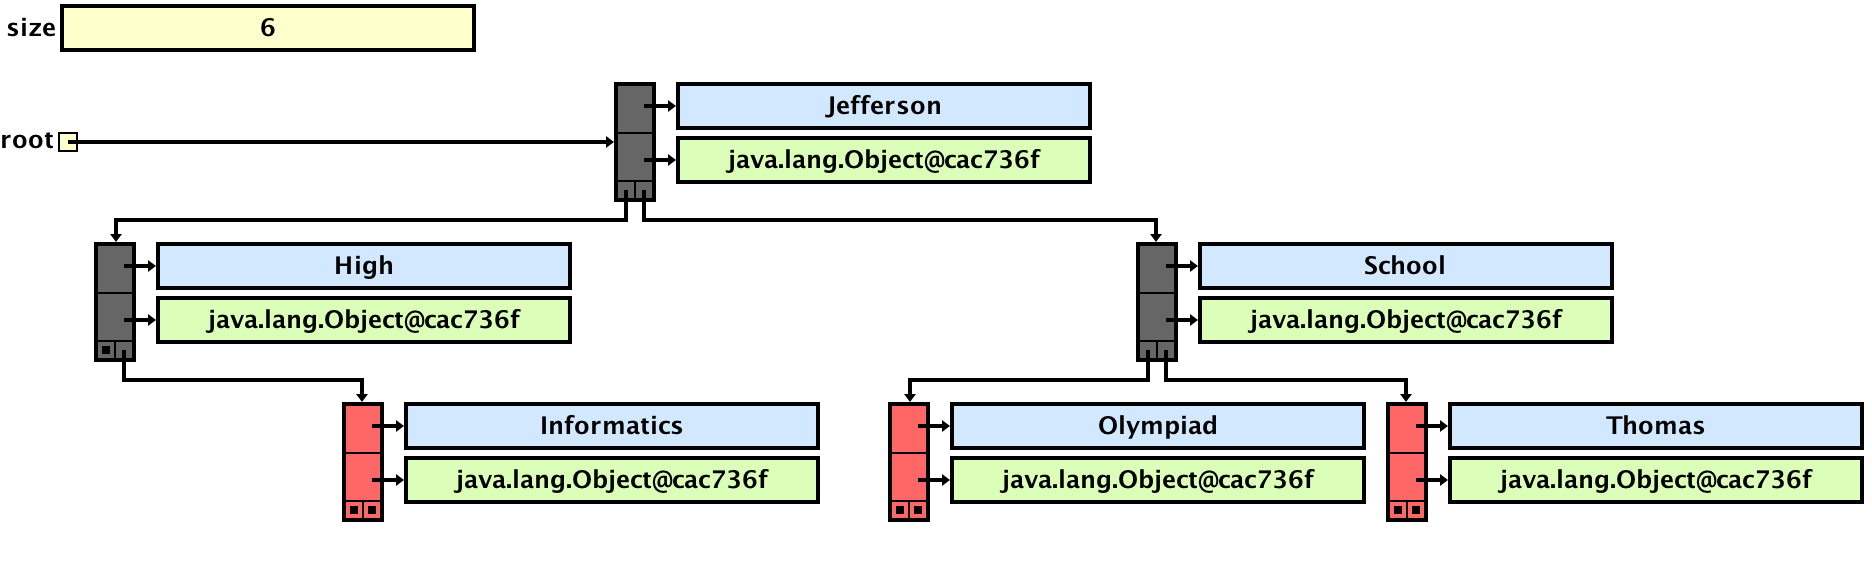
\includegraphics[scale=0.5]{treeset.png}


\subsection{Unordered Sets and Hashing}

A set without ordering is typically faster because of a widely-used trick known as Hashing. In brief, Hashing is a way of storing items so they can be found later on efficiently. The value itself is used to calculate the index it is stored in, to make it easier to search for later. To do this, the items are stored in a hash table at a position specified by a hash code. A hash code is an integer value calculated from any given data value or object, and is used to determine where a value should be stored in a hash table. This hash code value is generated by a hash function, which will always produce the same hash code given a specific data value or object. If two objects produce the same hash code, this is known as a collision. A collision is typically handled by creating buckets that contain LinkedLists - there is a list at each index, so that if more than one value happens to be stored there, it is added to the already existing list. If there is a collision and there is intent to do a look up, the run time would increase as the program would still have to go through all of the elements in the bucket. Unordered Sets use this trick to attain their $O(1)$ look up. In Java unordered sets are referenced as HashSets and in C++ they can be invoked by std::unordered\_set. In the representation below, you can see the hash table for this particular unordered set (notice the collision at index 0).

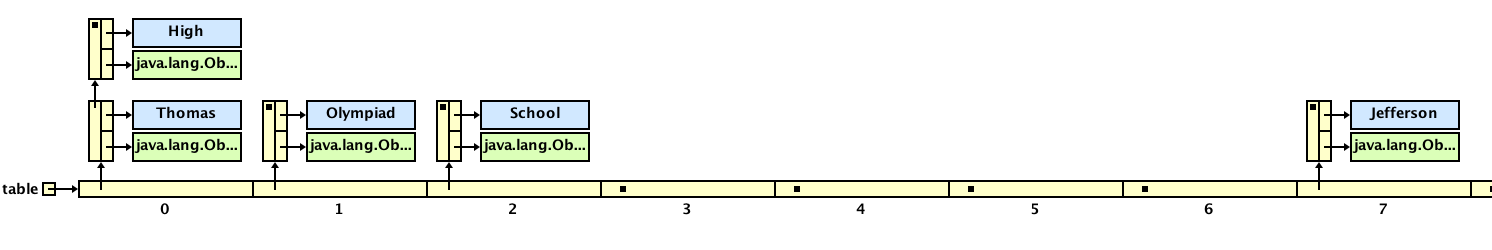
\includegraphics[scale=0.64]{hashset.png} 


